\subsection*{Soluzione es. 2}

Si riporta di seguito il listato dell'\emph{header file} che contiene
le dichiarazioni delle procedure che risolvono l'esercizio.
% zerofun.hpp
\lstset{basicstyle=\scriptsize\sf}
    \lstinputlisting[caption=Procedure per la ricerca
        degli zeri di una funzione.]{ex/1/zerofun.hpp}
\lstset{basicstyle=\sf}

Le corrispondenti definizioni sono state inserite nel \emph{source file}
\texttt{zerofun.cpp}:
\lstset{basicstyle=\scriptsize\sf}
    \lstinputlisting[caption=Procedure per la ricerca degli zeri di una
        funzione.]{ex/1/zerofun.cpp}
\lstset{basicstyle=\sf}

L'istruzione \texttt{assert(u*f(b)<0.0);} permette un semplice controllo degli errori,
perch\`e provoca l'interruzione del programma e la generazione di un
messaggio di errore se l'espressione \texttt{u*f(b)<0.0} non \`e verificata.

Infine riportiamo il listato contenente il main nel file \texttt{bn.cpp}:
\lstset{basicstyle=\scriptsize\sf}
    \lstinputlisting[caption=Definizione della funzione e main del programma.]
    {ex/1/bn.cpp}
\lstset{basicstyle=\sf}

Per la compilazione si ricorre ai seguenti comandi:
\begin{verbatim}
g++  -c -o bn.o bn.cpp -Wall
g++  -c -o zerofun.o zerofun.cpp -Wall
g++  -o bn bn.o zerofun.o
\end{verbatim}

I \emph{files} \texttt{bn.o} e \texttt{zerofun.o} sono la
rappresentazione in codice oggetto delle definizioni di tipi e
funzioni contenute nei \emph{files} sorgente
(rispettivamente \texttt{bn.cpp} e \texttt{zerofun.cpp}.
Il collegamento (\emph{linking}) dei \emph{files} oggetto
produce l'eseguibile \texttt{bn}.
Per disattivare tutti gli \cpp{assert} all'interno del codice,
in fase di compilazione occorre aggiungere il parametro \cpp{-DNDEBUG}
per quei files che utilizzano gli \cpp{assert}, ovvero
\begin{verbatim}
g++  -c -o bn.o bn.cpp -Wall
g++  -c -o zerofun.o zerofun.cpp -Wall -DNDEBUG
g++  -o bn bn.o zerofun.o
\end{verbatim}

Per visualizzare graficamente l'errore commesso, \`e possibile
aggiungere due parametri di input alle funzioni \texttt{bisection},
\texttt{newton} e \texttt{robust}.
Il primo \`e la soluzione esatta mentre il secondo \`e il nome del
file su cui salvare i dati.
Il listato dei comandi contenuti in \texttt{bng.cpp} \`e il seguente:
\lstset{basicstyle=\scriptsize\sf}
    \lstinputlisting[caption=Definizione della funzione e main del programma.]
        {ex/1/withGnuplot/bng.cpp}
\lstset{basicstyle=\sf}

Si noti il comando finale di chiamata al sistema operativo,
\`e richiesto quindi il file \texttt{print\_data} che contiene i seguenti comandi
\begin{verbatim}
set terminal png
set output "grafico.png"
plot "data" with lines
\end{verbatim}
I comandi in \texttt{zerofung.hpp} sono sostanzialmente identici a quelli
riportati in \texttt{zerofun.hpp}, mentre i comandi in \texttt{zerofung.cpp}
sono riportati qui di sequito
\lstset{basicstyle=\scriptsize\sf}
    \lstinputlisting[caption=Procedure per la ricerca degli zeri di una
        funzione.]{ex/1/withGnuplot/zerofung.cpp}
\lstset{basicstyle=\sf}

Si noti nella funzione \texttt{bisection} e \texttt{newton} la gestione del file.
Anzitutto viene dichiarato, dove \`e necessario l'operatore di scope resolution
\texttt{::} per accedere ai membri definiti nel namespace \texttt{std}.
Successivamente viene aperto in modalit\`a out nel caso della funzione
\texttt{bisection}, mentre in modalit\`a out e app nella funzione \texttt{newton}.
La differenza \`e che nel secondo caso i dati vengono scritti dal fondo del file.
Vi \`e poi un test per verificare se il file \`e stato effettivamente aperto.
All'interno di cicli vi \`e la scrittura dei dati, i comandi sono analoghi a
quelli utilizzati per la visualizzazione a schermo.
Alla fine di entrambe le funzioni il file viene chiuso.

Il grafico ottenuto \`e il seguente
\begin{figure}[!h]
    \centering
    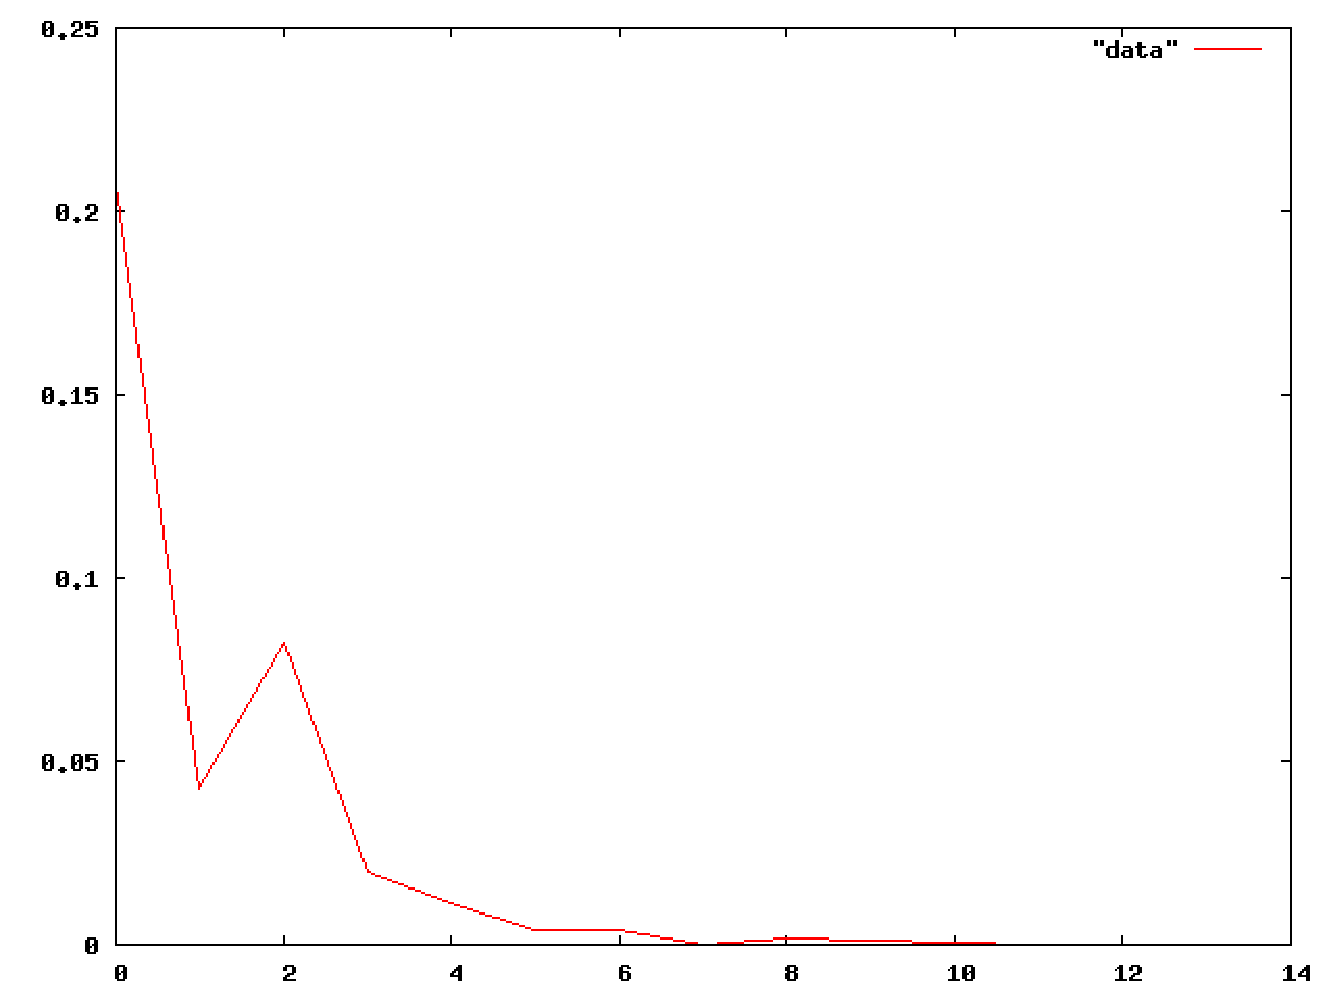
\includegraphics[width=0.7\textwidth]{./images/grafico}
\end{figure}
